\documentclass{amsart}
\usepackage[style=alphabetic,backend=biber,sorting=nty]{biblatex}
\addbibresource{biblio.bib}
\usepackage[T1]{fontenc}
\usepackage[french,english]{babel}
\usepackage[margin=0.6in]{geometry}
\usepackage{macros}
\usepackage{csquotes}
\usepackage{subfiles, caption, listings}
\usepackage[]{amsmath}
\usepackage{amssymb}
\usepackage{dsfont}
\usepackage{stmaryrd}
\usepackage{hyperref}
\usepackage{graphicx}
\usepackage{varwidth}
\usepackage{float}
\usepackage{amsthm}
\usepackage{verbatim}
\usepackage{enumitem}
\usepackage[most]{tcolorbox}
\usepackage[ruled]{algorithm2e}
\usepackage{relsize}
\usepackage{mathtools}
\usepackage{csquotes}
\usepackage{wrapfig}
\usepackage[colorinlistoftodos]{todonotes}
\renewcommand\thesection{\arabic{section}}

\newcommand{\lref}[1]{\mbox{\thref{#1}}}

%THEOREMS
\theoremstyle{definition}
\newtheorem{definition}{Definition}

\theoremstyle{plain}
\newtheorem{theorem}{Theorem}
\newtheorem{lemma}{Lemma}

\setlist[enumerate,1]{label={(\roman*)}}

\date{December 20, 2024}
\title{Waltz right turn with a Humanoid Robot using Inverse Kinematics}
\author{Constantin Vaillant-Tenzer, Charles Monté}

\begin{document}

\maketitle


\section{Introduction}

% TODO @Constantin: Relire, corriger et etoffer si besoin

Our goal was to code a robot able to dance a waltz right turn using inverse kinematics. To do so, we first implemented a movement acquisition pipeline adapted from various research papers to get the position of joints of interest (feet, pelvis, hands, and head) over time. We then used the joint positions to solve inverse kinematics on a humanoid robot, forcing the robot's joints to follow the ideal positions. Finally, we adapted the rhythm of the movement to fit the BPM of a chosen music.

\section{Previous works}
Waltz dancing is not a common research topic among dancing robots. However, to help robots learn how to dance, there are some already known methods like \textbf{learning from observation}\cite{traditional_jap_dance} where the robot chooses from a series of leg tasks the good ones to imitate a dancing human; or \textbf{real-time gesture responsive frameworks}\cite{spectacle_imitation} where the robot generates unpredictable artistic responses to a dancer's movements.

Concerning waltz dancing, a \textbf{dance partner robot}\cite{ballroom_dance} has been developed to realize human-robot coordination by estimating the next intended movement of a human through physical interaction.

\section{Theory behind the movement}

% TODO @Constantin: Relire, corriger et etoffer si besoin

The movement made during a right turn of the waltz dance can be well described using the movement of the center of gravity of the person dancing. \\ 

During the dance, the person's movement is split in two summed parts: while moving along the perimeter of an ellipse - most commonly referenced as \textbf{the ball circle} - the dancer turns on himself along the perimeter of a circle with a diameter close to 1 meter.\\

Both those translations can be estimated to be of constant angular velocities. \\ 

The dancer does a full turn around the circle every 360 beats of the music (of known BPM) so the angular velocity around the circle is $\omega_C = \frac{-2\pi \text{BPM}}{6*60}$ while we estimate the dancer to go around the ball room every minute, meaning the angular velocity around the ellipse is $\omega_E = \frac{-2\pi}{60}$. \\ 

The movement of the center of gravity we aim at reproducing is depicted in Figure~\ref{fig:cog_movement}

\begin{figure}
  \centering
  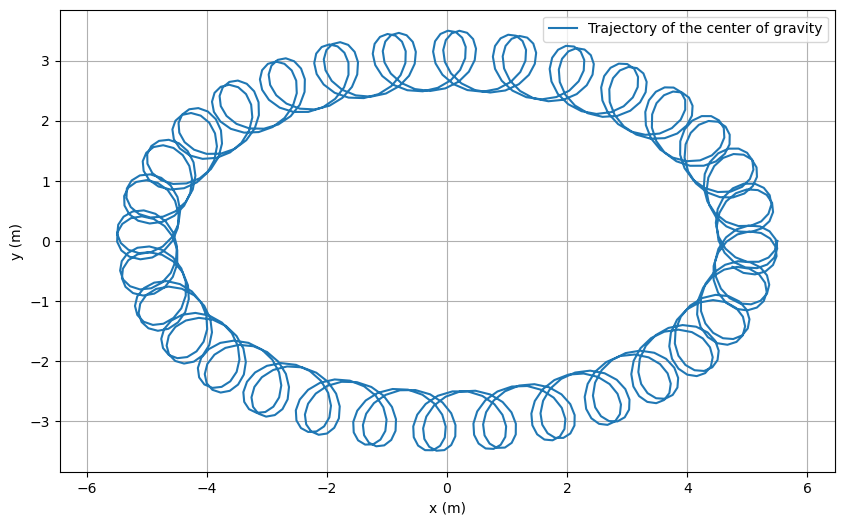
\includegraphics[width = 0.5 \columnwidth]{img/waltz_cog_movement.png} 
  \caption{Simulated movement of a Waltz dancer's center of gravity for 2 minutes}\label{fig:cog_movement}
\end{figure}

\section{Our method}

% TODO @Constantin: Relire, corriger et etoffer si besoin

\subsection{Overview of the method}
To simulate the trajectory done by a dancer with a robot, we have trained a humanoid robot to follow the sequence of movements done by the dancer during a waltz right turn. \\

To do so, we first had to make the assumption that gravity and other forces applied to the dancer does not affect their movement. We also decided to mainly focus on how well the joints would follow the movement, without centering ourselves on physical constraints like making sure that the robot's feet are always on the ground.\\

To acquire the kinematics of the waltz right turn with the help of a video and then solve inverse kinematics with a humanoid robot model to fit the acquired movement. 
After having a robot able to dance the waltz right turn, we only had to fit the robot's movement to the music BPM, by making sure a right turn had the right duration.\\

We did not have sufficient time to implement everything ourselves from kinematics acquisition to inverse kinematics solving so we decided to center ourselves around acquiring a good base for the movement kinematics. \\

Thus, we mainly relied on already implemented blocks to fit inside our pipeline while trying to get the best approximation of a waltz right turn possible.\\

The global pipeline we followed for our implementation is represented in Figure~\ref{fig:pipeline}.

\begin{figure}
  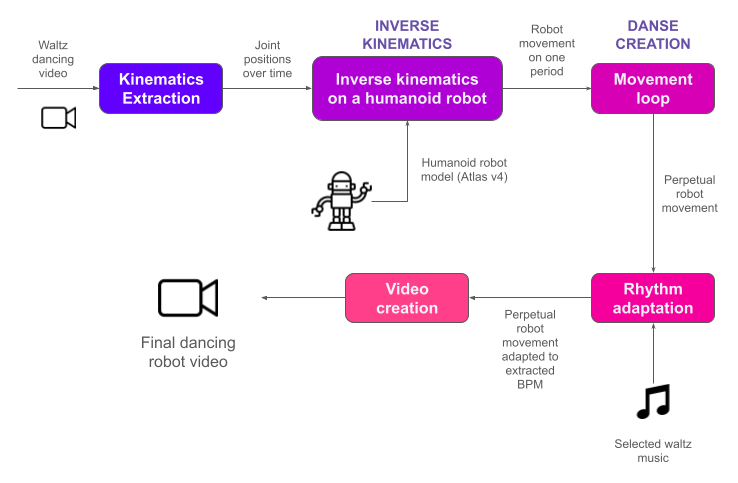
\includegraphics[width = 0.75 \columnwidth]{img/final_solution_pipeline.png}
  \caption{Our approach's full pipeline}\label{fig:pipeline}
\end{figure}

\subsection{Kinematics Extraction}
Our first idea of Kinematics Extraction was to both extract joint positions and joint angles, to ensure a perfect movement for the robot throughout the waltz movement. This idea did not work in the end, which made us go back to only joint position extraction while putting no constraints on the robot's joint angles, to make the inverse kinematics process find the optimal joint angles itself. In this subsection, we are going to chronologically follow our thought process and implementations of kinematics extraction.\\

We first decided to focus on two methods, one was proposed by Stéphane Caron at the start of the project : Estimating 3D Motion and Forces of Person-Object Interactions From Monocular Video\cite{Li_2019}, and the second was discovered during research about state-of-the-art kinematics extraction algorithms: NIKI, Neural Inverse Kinematics with Invertible Neural Networks for 3D Human Pose and Shape Estimation\cite{li2023niki}.\\

We did not focus long on the first method as its implementation was made using outdated projects (HMR for instance) which made the global implementation too tiresome. NIKI on the other hand was perfect for us, as it extracted both the joint positions and the joint angles at the same time. While the joint positions were easy to understand and use (with some tinkering to find each Joint Id - see NIKI results exploitation notebook in the GitHub), the joint angles did not follow a shape we understood. We were provided with fewer angles than the number of joints and no idea of which joint they were related to. We did not manage to understand how to extract each joint's angle over time, even after carefully reading the related paper and source code. \\

\begin{figure}
  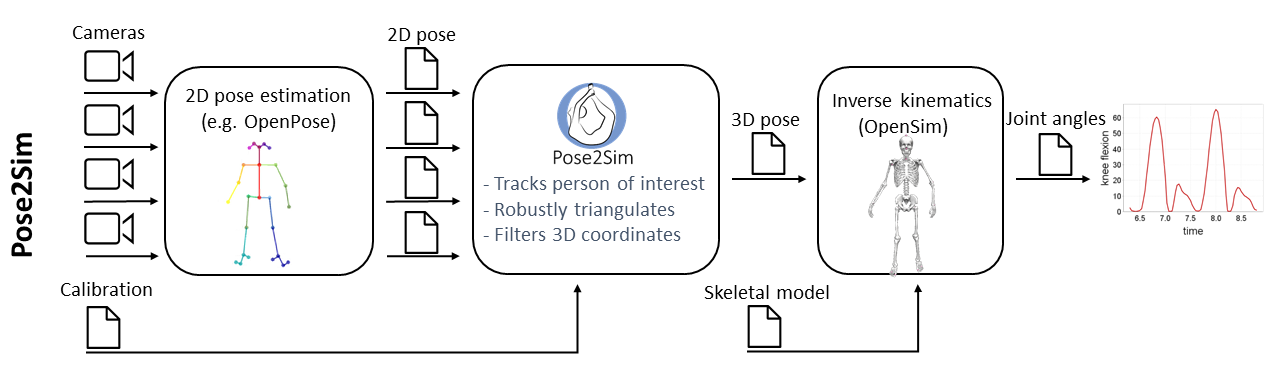
\includegraphics[width = 0.99 \columnwidth]{img/pose2sim_pipeline.png}
  \caption{The Pose2Sim pipeline : This solution extracts 2D keypoints coordinates (using RTM Pose\cite{RTMPose}) to produce an OpenSim result (full-body 3D joint angles), which we use in our pipeline by extracting the information that is interesting from us, ie. the RTMPose output and the full-body 3D joint angles.}\label{fig:pose2sim_pipeline}
\end{figure}

Thus, we decided to find a new pipeline that could extract both, in an intelligible manner: Pose2Sim\cite{Pose2Sim}. Pose2Sim has been the main pipeline we have used for the extraction of joint positions and angles, mainly because the outputs were directly linking each joint name to an angle and a position. Pose2Sim's global pipeline can be found in Figure~\ref{fig:pose2sim_pipeline}. This solution is not that different from the two proposed above, they follow a similar chain of thought which consists of a 2D pose estimation algorithm (RTM Pose\cite{RTMPose} for Pose2Sim), followed by a block that projects those coordinates to the 3D space, before doing inverse kinematics to find the optimal joint angles to adapt the joint positions to a humanoid model. \\

Even if only using the first part of all those implementations to extract the 3D joint positions before using our own Inverse Kinematics to get the optimal joint angles now seems obvious, we lost a lot of time trying to use both the joint positions and angles to try and get a perfect movement. We first implemented a global pipeline using the Pose2Sim results, which we presented during the poster session. It did not work due to bad adaptations of the joints to the angles and the positions, which blocked the robot in place, only allowing its feet to move. \\

After reflecting on our implementation, we managed to make the robot move but noticed that both the Pose2Sim and NIKI extracted joint positions were not parallel to the $(x, y)$ plane. Thus, we decided to find optimal transformation matrices (composition of rotations, translations, and scaling for the $x$, $y$, and $z$-axis) but did not manage to find one, manually or with optimization algorithms, to make Pose2Sim results exploitable. The reasons we identified for it were two-fold.

\begin{enumerate}
    \item The transformation applied to the movement was too difficult for us to estimate manually and we did not manage to find optimal cost algorithms to have a good transformation matrix output.
    \item The Pose2Sim pipeline adapts the joint positions to the 3D space with the use of the extrinsic and intrinsic camera parameters while assuming that the camera is static. However, in the video we used, the camera moves during the acquisition which throws off the Pose2Sim estimation causing a huge change in $x,y,z$ coordinated in the middle of the movement, as seen in Figure~\ref{fig:x_coord_pose2sim}.
\end{enumerate}
\begin{figure}
  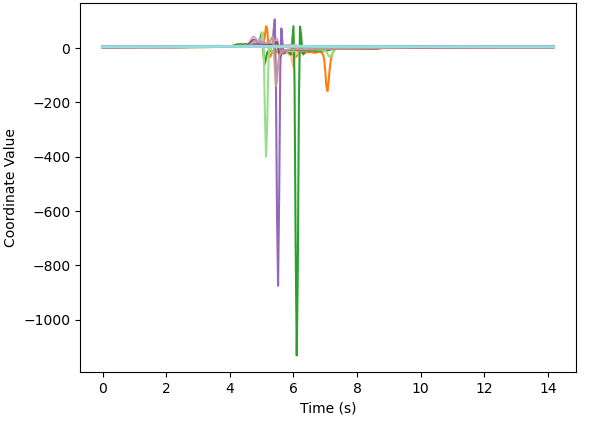
\includegraphics[width = 0.33 \columnwidth]{img/x_coord_pose2sim.png}
  \caption{x-coordinate of each joints over time with Pose2Sim extraction}\label{fig:x_coord_pose2sim}
\end{figure}
\begin{figure}
  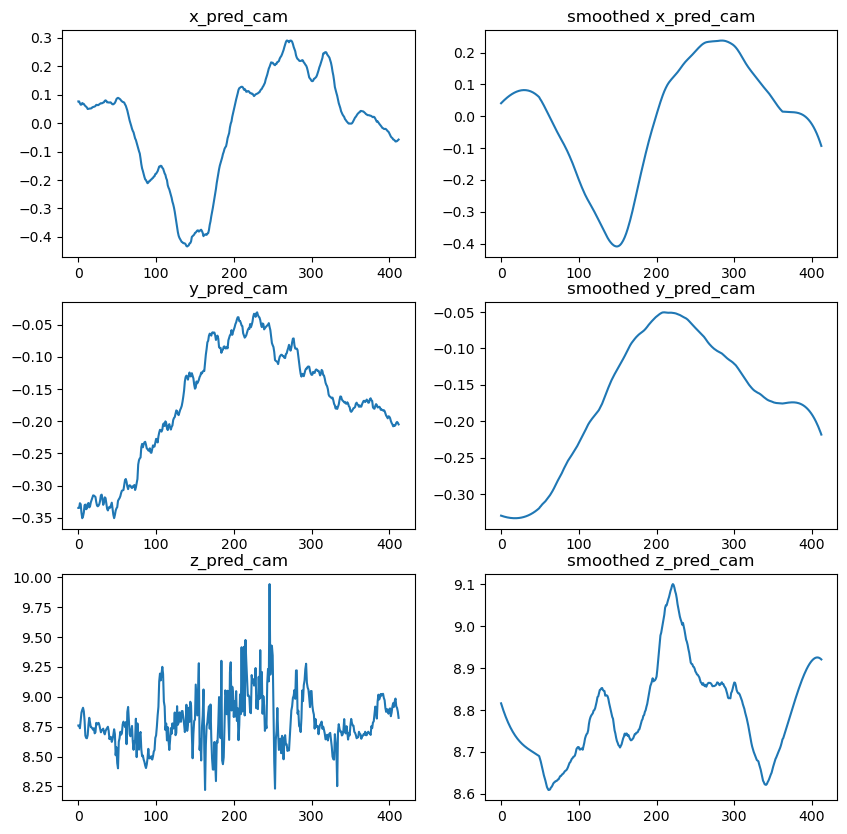
\includegraphics[width = 0.5 \columnwidth]{img/influence_of_smoothing.png}
  \caption{Influence of smoothing on the coordinates of the pelvis joint over time}\label{fig:influence_of_smoothing}
\end{figure}
\begin{figure}
  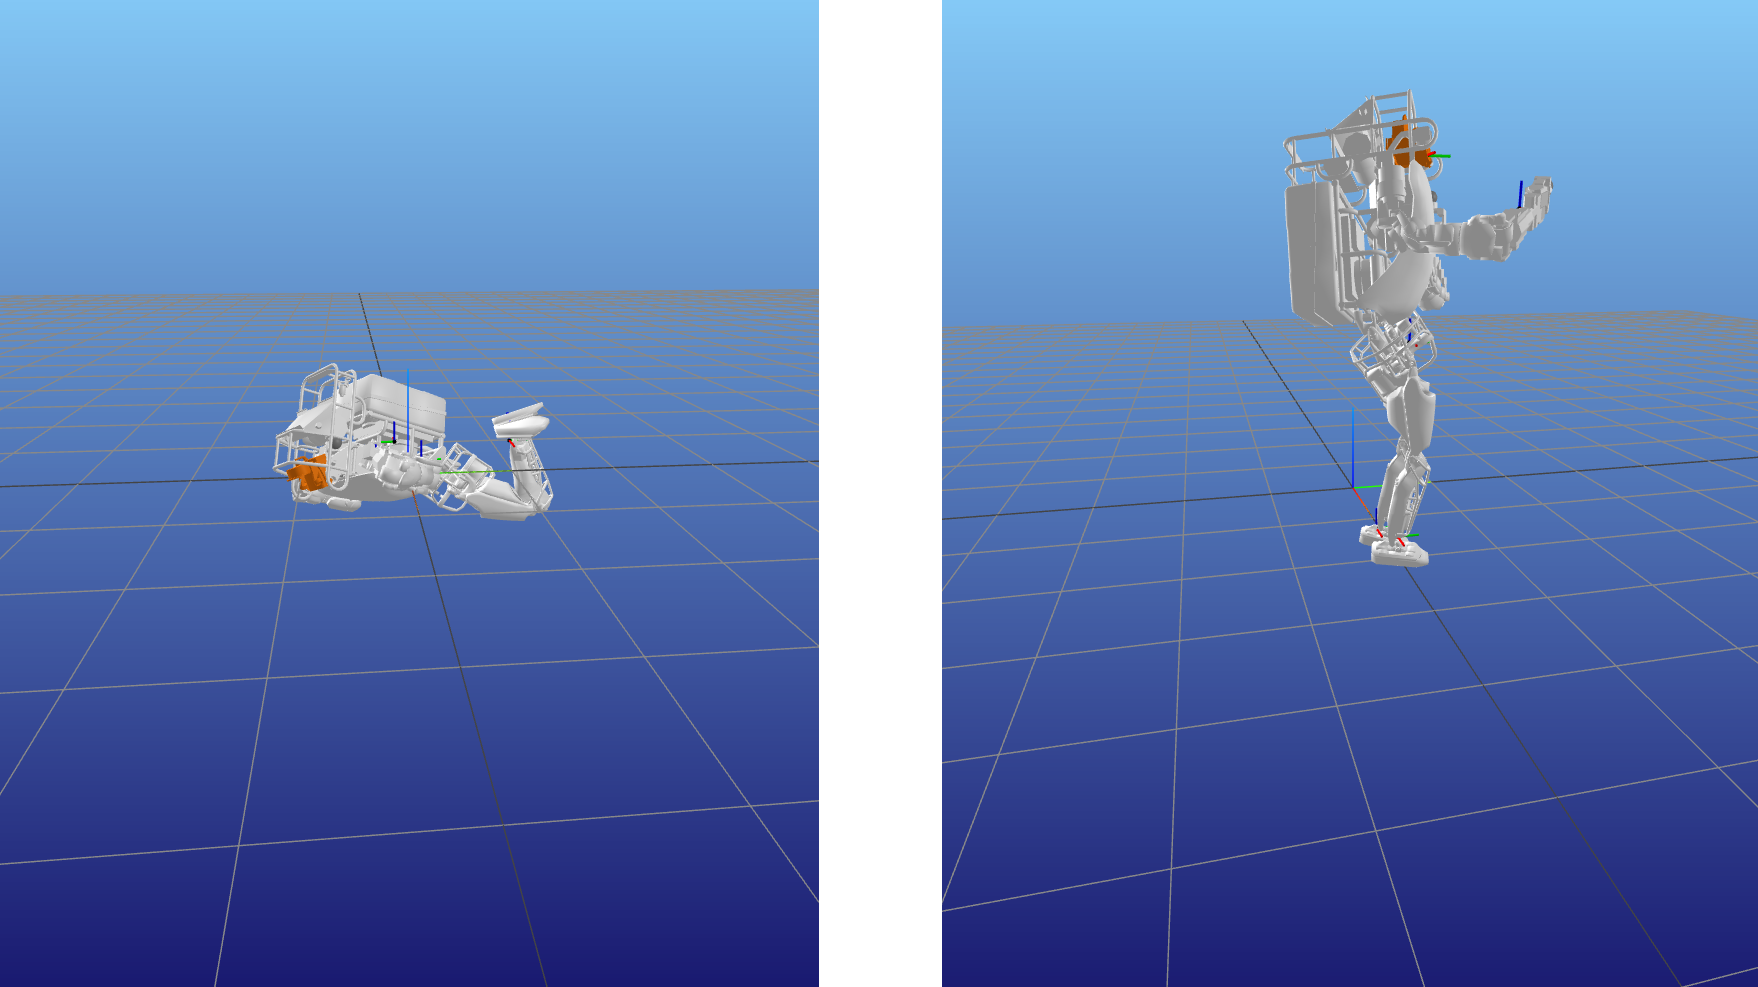
\includegraphics[width = 0.75 \columnwidth]{img/influence_transformation.png}
  \caption{Influence of the transformation stage. Left: Before transformation, Right: After transformation}\label{fig:influence_transformation}
\end{figure}

Looking at all the extraction we had made, we concluded that NIKI's way of extracting joint positions, based on a CNN backbone output robust to camera movements which is then enhanced by the NIKI solver (which is an Invertible Neural Network for Inverse Kinematics solving), was the best solution for us to extract the joint positions. Only using the joint positions extracted thanks to the NIKI algorithm, pre-processing them using smoothing functions for each coordinate and making them parallel to the $(x, y)$ plane worked for us. The main reason why NIKI performed better for us was because the transformation matrix was easier to find and the joint positions were more stable over time.\\

The smoothing part was important as we noticed a lot of noise on the prediction of the center of mass' position, especially in the $z$-axis. However, this position was directly used as the position of the pelvis joint and added to each joint position to make the robot move in the 3D space and avoid it being anchored at the origin. The use of smoothing was crucial for our implementation, as the noise was highly impacting the quality of the feet's movement. To reduce it, we used a savgol filter to smooth the coordinates, its influence can be seen in Figure~\ref{fig:influence_of_smoothing}.\\

The transformation of the coordinates to make them parallel to the $(x, y)$ plane discussed earlier has been done by finding the optimal rotation matrix that would make the pelvis joint's $z$-coordinate equal to half the robot's height. We did not manage to find a way to do it automatically so we had to find the optimal rotation matrix manually. The influence of the transformation can be seen in Figure~\ref{fig:influence_transformation}.\\

We then only had to solve the inverse kinematics using those joint positions to find the optimal angles automatically.

\subsection{Choice of the robot}

% TODO @Constantin: Ajouter pourquoi on a choisi AtlasV4 + Relire, corriger et etoffer si besoin

We explored the Robot descriptions in Python repo\cite{robot_descriptions_py} to find a humanoid robot with similar joints to our Pose2Sim output, we finally decided to use AtlasV4 as our humanoid model because...

\subsection{Inverse Kinematics}
To solve the inverse kinematics, we applied Pink\cite{pink2024} which solves differential inverse kinematics by weighted tasks. \\

The method uses residual functions of the robot configuration $q$ that should be driven to zero to make the robot do a certain task. In our case, we for instance try to put the robot's feet at a certain position $p_{\text{feet}}^*$ so an example of a residual would be $e(q) = p_{\text{feet}}^* - p_{\text{feet}}(q)$. \\

To solve the equation system produced, the method computes a velocity $v$ that satisfies the equation $J_e(q)v = \dot{e}(q) = -\alpha e(q)$ - $J_e(q)$ being the Jacobian of task $e$ - for each residual. 
It is of course not possible so the method finds the optimal solution to the following minimization problem, which finds the movement that best solves all of the tasks at the same time.
$$
\begin{aligned}
\min_v \ \ &\sum_{\text{tasks} \ e} ||J_e(q)v + \alpha e(q)||^2 \\
\text{subject to} \ \ \ &v_{min}(q) \leq v \leq v_{max}(q)
\end{aligned}
$$\\

Regarding the python side of things, as Pink revolves around the introduction of tasks, we had to choose which tasks we wanted to solve. We decided to focus on the feet, pelvis, hands, and head, as they are the most important parts of the body for a waltz right turn. \\

We forced all those joints to follow the positions extracted from the NIKI pipeline using FrameTasks, which are tasks that force a certain frame to follow a certain position and orientation. To keep the robot steady, we added a PostureTask that forces the robot to stay in a certain posture, which we chose to be the initial posture of the robot.\\

Concerning the weights, we decided to put all the weights on the joint orientations to 0, and only play on the weights of the joint positions. We decided to put the weights of the feet, the pelvis and the head higher than the weights of the hands, as the hands are not as important as the other parts of the body for a waltz right turn, but are necessary to ensure a rotation of the robot's body.

\subsection{Rhythm adaptation}

To adapt the rhythm of the movement to the BPM of the music, we simply decided to calculate the ideal time between each frame of the movement to adapt it to the BPM of the music. \\

To do so, we calculated the time it would take the robot to do 4 full turns around the small circle at the new BPM (as Constantin does 4 full turns during the video) and divide the number of frames by this time to get the new ideal frame rate. The new ideal time between each frame is then the inverse of this frame rate.\\

\section{Our results}

% TODO @Constantin: Ecrire toute cette partie
% J'ai pensé à plusieurs choses à montrer dans cette partie :
% - Montrer les résultats de la méthode en 2D avec le graph vu de haut
% - Montrer les résultats de la méthode en 3D avec le robot qui danse (donner lien de vidéo youtube dans le rapport et ajouter des images du robot qui danse ?)
% - Montrer les résultats de l'adaptation du rythme à la musique ?

\section{Next steps}

% TODO @Constantin: Ecrire toute cette partie, j'ai rajouté ce qu'on avait mis dans le poster, à voir si on veut réécrire ou rajouter des choses

While the results already are satisfying, we identified two further steps that could be added to the pipeline to achieve even better results :
\begin{enumerate}
    \item Adding a controlling module to maintain a constant angular velocity on the small circle. This cannot be done by humans and will make the movement look even better.
    \item Take care of the robot's balance throughout the movement;
    \item Be able to dance the waltz right turn with a partner.
\end{enumerate}

\section{Conclusion}

% TODO @Constantin: Ecrire toute cette partie
% Dans l'idée je pense qu'il faudrait juste essayer de répondre aux problématiques dans l'introduction, quitte à quasi la répéter

\printbibliography[]

\end{document}